\documentclass{article}
\usepackage{graphicx}
\usepackage{float}
\usepackage[acronym]{glossaries}
\usepackage{fullpage}

\loadglsentries{acronyms}
\makeglossaries

\begin{document}

\begin{tabular}{rl}
  \textbf{Lab 8:} & DC Generators \\
  \textbf{Performed:} & March 26, 2013 \\
  \textbf{Partners:} & Rawley Dent \\ & Charles Pittman \\
  \textbf{Instructor:} & Dr. Weatherford
\end{tabular}

%\setlength\parindent{0pt}

\section*{Abstract}

In this experiment, the effect of a DC motor's construction on its torque-speed
relationship (also referred to as its terminal characteristics) was examined.
The three connection types examined here are: series-connected,
shunt-connected, and compound-connected (a combination of the two).

\section*{Results}

\begin{figure}[H]
  \centering
    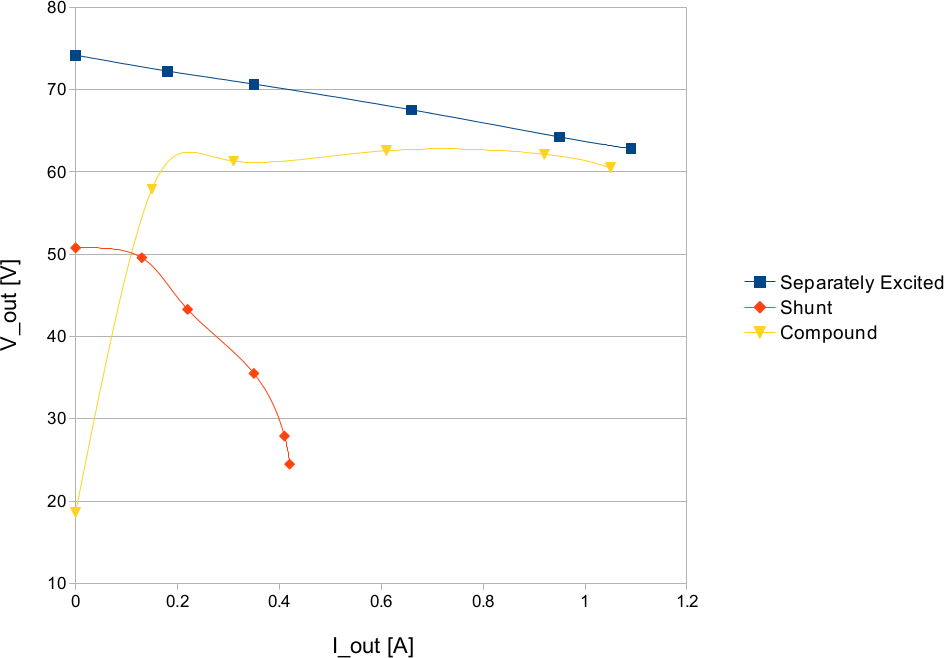
\includegraphics[width=0.8\textwidth]{img/graph}
    \caption{\textbf{Comparison}}
    \label{fig:graph}
\end{figure}

\section*{Conclusions}

The torque-speed relationship, or terminal characteristics, of the shunt motor
resembles a straight line. In fact, the equation for a shunt motor’s
torque-speed relationship is linear, with a negative slope. The terminal
characteristics of a series motor are nonlinear. It is noted that as the torque
on a series motor goes to zero, its speed goes to infinity.  However, the
torque on a motor can never go to zero because of the mechanical, core, and
stray losses that must be overcome. Just as well, the speed of a series motor
can still turn fast enough to damage itself. The terminal characteristics of a
cumulatively compounded motor resemble both a series and a shunt motor. This is
because the compounded motor contains both a shunt and a series field. Although
the resemblance is hard to discern from Figure~\ref{fig:graph}, if more data
was obtained, it would be apparent that the motor resembles a shunt motor at
low torques, and a series motor at higher torque.

\end{document}
